%%%%%%%%%%%%%%%%%%%%%%%%%%%%%%%%%%%%%%%%%
% Capture the flag Writeup Template. 
% LaTeX Template
% Version 1.0 
%
% This template has been downloaded from:
% http://www.latextemplates.com
%
% Original authors:
% Hector F. Jimenez S. <hfjimenez@utp.edu.co>
% Pereira Security Team 2013.
% License:
% CC BY-NC-SA 3.0 (http://creativecommons.org/licenses/by-nc-sa/3.0/)
%
%
%----------------------------------------------------------------------------------------
%	PACKAGES AND OTHER DOCUMENT CONFIGURATIONS
%----------------------------------------------------------------------------------------
\documentclass[a4paper]{article}
\usepackage[spanish]{babel}
\usepackage[utf8x]{inputenc}
\usepackage[T1]{fontenc}
\usepackage{amsmath,amsfonts,amsthm} 					% Math packages.
\usepackage{graphicx}
\usepackage{float}										% Image will be in the same place as you want.!!! x-/
\graphicspath{ {./img/} }							% Where to look for the images.
\DeclareGraphicsExtensions{.pdf,.png,.jpg}				% Graphics Extension to be used
\usepackage{url}
\usepackage{color}
\usepackage{hyperref}
\hypersetup{
    colorlinks,
    citecolor=black,
    filecolor=black,
    linkcolor=black,
    urlcolor=blue
}
\newcommand\fnurl[2]{%									% set a simple and quick footnote command and include url.
\href{#2}{#1}\footnote{\url{#2}}%	
}
\usepackage{minted}										% For syntax highlighting.
\usepackage[export]{adjustbox}
\usepackage{geometry}
 \geometry{
 a4paper,
 total={210mm,297mm},
 	left=30mm,
 	right=20mm,
 	top=20mm,
 	bottom=20mm,
 	bindingoffset=0mm
 }
 

\title{}
\author{												% Authors begin.
Héctor F. \textsc{Jiménez S.}\\
\texttt{hfjimenez@utp.edu.co} \\
\and
Sebastian \textsc{Zapata}\\
\texttt{sebastzapata93@gmail.com }\\
\and 
Juan Francisco \textsc{Gallego}\\
\texttt{juanfran16@utp.edu.co}
} 		\begin{document}
\begin{titlepage} 				
\begin{center}	  				
\vfill
\line(1,0){250}\\ 			
\huge\textbf{Desarrollo de un Turnero Digital\\ 
Usando FPGA's}\\
\Large{ Laboratorio de Electrónica Digital}\\
\Large{ Reporte Final} \\
\line(1,0){250}\\
\vspace{3em}	
\large{Francisco Gallego Leon}\\
\texttt{CC.\textit{1088336670}}\\
\large{Héctor F. Jiménez Saldarriaga}\\
\texttt{CC.\textit{1115421345}}\\
\large{Sebastian Zapata Ruiz}\\
\texttt{CC.\textit{1088313682}}\\
\vspace{3em}															
\large{Prf. Ramiro Andrés Barrios Valencia }\\
\end{center}
\vspace{2em}
\centerline{\includegraphics[scale=0.3]{img/portada}} 
\vspace{5em}				
\begin{center}
\large{Facultad de Ingenierías, \\ Ingeniería de Sistemas y Computación }\\
\vspace{1em}
\large{Universidad Tecnológica de Pereira}\\
\vspace{2em}				
\large{2016-2}
\end{center}
%Espacio entre imagen e imagen


\vspace*{\stretch{2.0}}
\end{titlepage}
																			%Pagina En blanco
\clearpage
    \thispagestyle{empty}
    \phantom{a}
    \vfill
    \begin{center}Pagina Dejada Intencionalmente en Blanco\end{center}
    \vfill
\newpage
\tableofcontents
\newpage
\clearpage
\maketitle
\begin{abstract}
En el presente documento se refleja el trabajo realizado para llevar a cabo el generador de turnos, el desarrollo de este proyecto fue llevado a cabo en 5 etapas durante el transcurso del semestre, el objetivo principal que se buscaba con este, era construir un dispositivo de apoyo a las entidades que tiene que atender demasiadas personas simultaneas. 
Para poder lograrlo durante el semestre los integrantes cada uno se encargaron de tareas y módulos específicos facilitando que cada integrante desarrollara sus fortalezas. 
\end{abstract}

La arquitectura de los proyectos es la siguiente:

\begin{figure}[H]
  \centering
     \includegraphics[width=0.7\textwidth]{generadorturnos}
  \caption{Generador de Turnos, esquema general.}
      \label{fig:debounce}
\end{figure}

\begin{figure}[H]
  \centering
     \includegraphics[width=0.5\textwidth]{panoramageneral}
  \caption{Mesas del turnero.}
      \label{fig:debounce}
\end{figure}

\clearpage
\newpage
%Modulo Antirebote.
\section{Modulo 1: Anti-rebote\label{antirebote}}
Utilizar switches y pulsadores mecánicos en un sistema electrónico es una práctica muy común, pues sirven de interfaces entre el usuario y el sistema embebido para seleccionar y programar funciones que este posee; en la práctica actual muchos de estos sistemas mecánicos están siendo reemplazados por displays táctiles pero hay situaciones industriales principalmente en las cuales un pulsador mecánico sería una solución más apropiada y eficiente en la implementación, pues al ser un sistemas mecánicos estos no se degradan tan rápido como lo harían las pantallas táctiles en un entorno industrial. Una de las grandes desventajas que poseen los pulsadores son los rebotes o saltos como se puede observar en la figura \ref{fig:debounce}.\\
\begin{figure}[H]
  \centering
     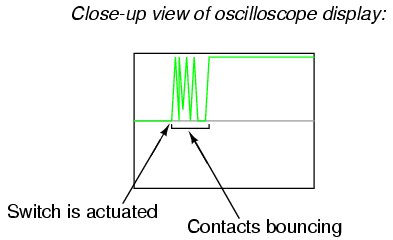
\includegraphics[width=0.7\textwidth]{debounce}
  \caption{Rebotes al presionar un pulsador mecánico, señales de osciloscopio.}
      \label{fig:debounce}
\end{figure}
Los elementos mecánicos del pulsador están constituidos por un par de contactos eléctricos que se unen o separan por medios mecánicos,  en la figura \ref{fig:pulsador} se muestra un pulsador común, figuras\ref{fig:pulsadorinternal1} \ref{fig:pulsadorinternal2} son vista detalladas. Los falsos contactos que se producen cuando los accionamos, crean falsas señales instantáneas, ocasionando un mal funcionamiento del dispositivo, no olvidando mencionar que existe una barrera o GAP que se produce por el aire entre los elementos mecánicos\textit{( aunque típica mente esto es despreciable por su baja fuerza discipativa)} induciendo múltiples pulsaciones o flancos como se muestra en la figura \ref{fig:debounce}. 
\begin{figure}[H]
  \centering
     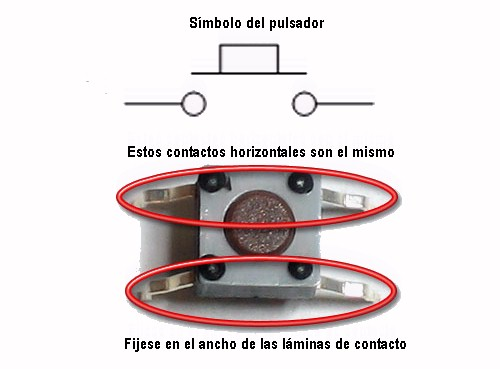
\includegraphics[width=0.5\textwidth]{pulsador}
  \caption{Pulsador Común, Composición.}
      \label{fig:pulsador}
\end{figure}

\begin{figure}[H]
  \centering
     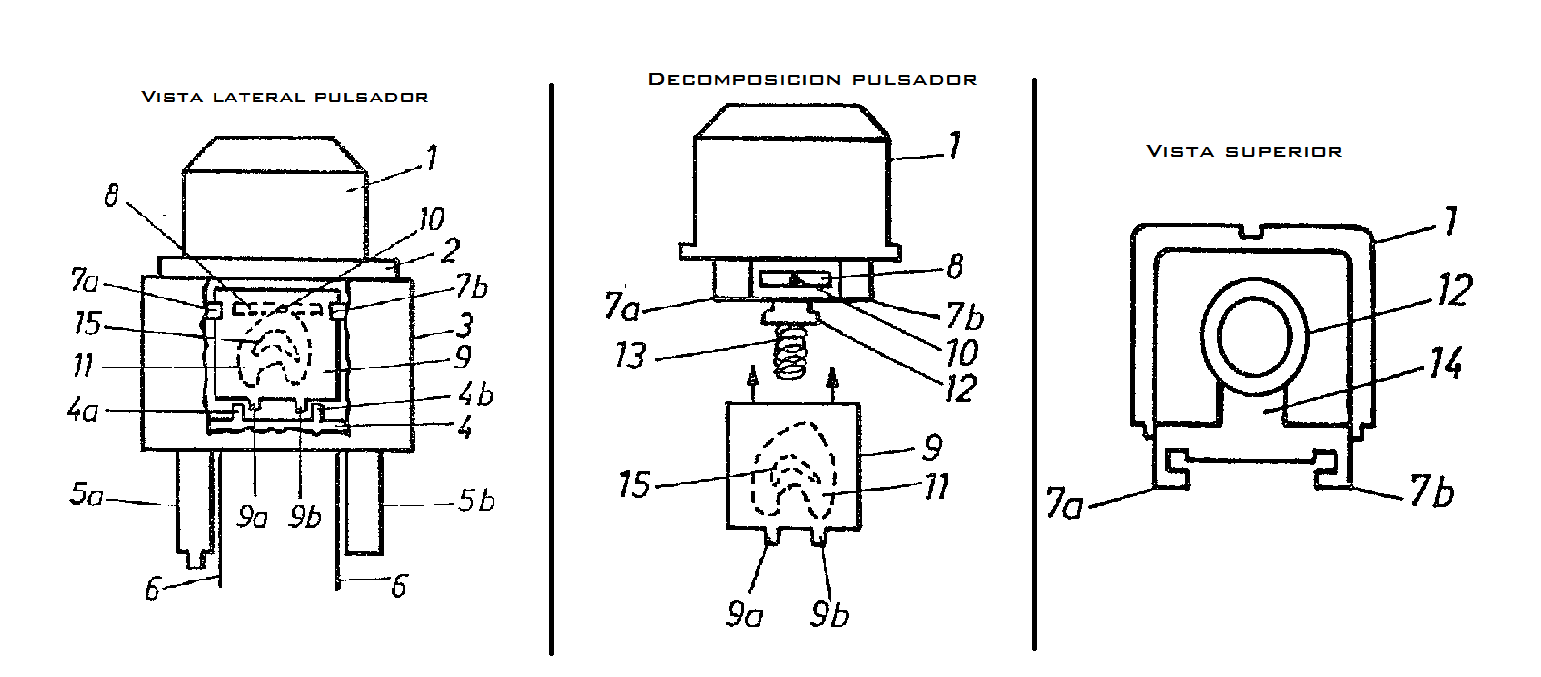
\includegraphics[width=0.7\textwidth]{pulsadorinternals}
  \caption{Decomposicion de un Pulsador común}
      \label{fig:pulsadorinternal1}
\end{figure}
\begin{figure}[H]
  \centering
     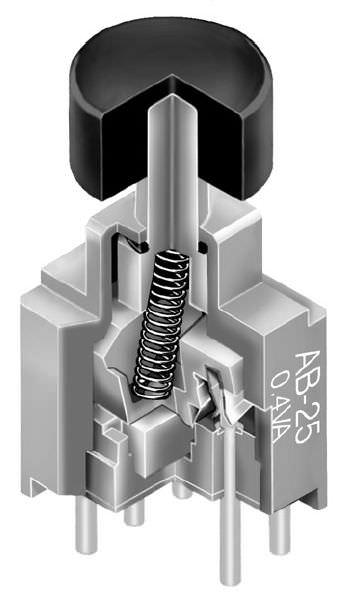
\includegraphics[width=0.2\textwidth]{internal}
  \caption{Vista en 3d de un pulsador y sus elementos }
      \label{fig:pulsadorinternal2}
\end{figure}
\label{sec:pulsador} 
En algunos casos esta acción puede producir una chispa debido a la corriente que atraviesa los contactos, disminuyendo el tiempo útil de los contactos eléctricos. La chispa se produce siempre al separar los contactos (desconectar), en ocasiones parece que también salta al conectarlos, eso es debido a los rebotes mecánicos que se producen al cambiar de estado.
Existen muchas formas de lidiar con este problema, tanto soluciones por hardware físico como el circuito simple de la figura \ref{fig:hardwc} o por software como lo realizaremos para el desarrollo de este modulo, mediante la implementación de un circuito lógico provisto por la empresa \fnurl{Digikey.}{http://www.digikey.com/}\\
\begin{figure}[H]
  \centering
     \includegraphics[width=0.7\textwidth]{debouncecircuit}
  \caption{Solución utilizando un simple arreglo electrónico. Pulsadores con resistencias de Pull Ups.}
      \label{fig:hardwc}
\end{figure}
\subsection{Arquitectura de la Placa \emph{NEXYS 2}}
La tarjeta de entrenamiento \emph{NEXYS 2} es una plataforma de desarrollo fabricada por la empresa \footnote{Digilentinc Página Oficial \fnurl{Nexys2 Spartan3E}{http://store.digilentinc.com/nexys-2-spartan-3e-fpga-trainer-board-retired-see-nexys-4-ddr/}} aunque se encuentra descontinuada para la venta y recomiendan utilizar esta misma en su versión \textbf{4}, utiliza una fpga Spartan 3E optimizada para desarrollo de aplicaciones donde se requiere implementar diseños de lógica compleja, e ideal para el procesamiento de señales y desarrollo de sistemas embebidos como se menciona en \fnurl{General Spartan Versions}{http://www.xilinx.com/support/documentation-navigation/silicon-devices/mature-products/spartan-3e.html}, \fnurl{Spartan-3E FPGA Family: Introduction and Ordering Information}{http://www.xilinx.com/support/documentation/data_sheets/ds312.pdf}.
\\Algunos elementos destacables de la placa son :
\begin{description}
  \item[Connectores] \hfill \\
  	\begin{itemize}
		\item Puerto USB2.0
	    \item Puerto VGA
		\item PS/2
	    \item Puerto RS232
    \end{itemize}
\begin{figure}[H]
 \centering
   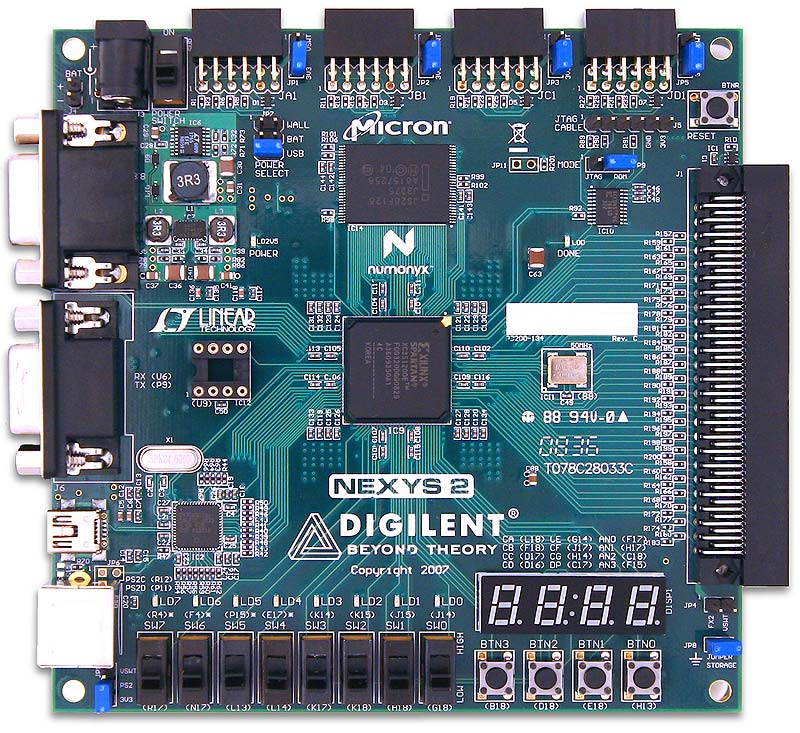
\includegraphics[width=0.7\textwidth]{model}
 \caption{Modelo de la Nexxys , Versión 2.}
    \label{fig:modelo}
\end{figure}
Algunas de las que más nos llamaron la atención son:\\
  \item[Caracteristicas] \hfill \\
    	\begin{itemize}
			\item Xilinx Spartan-3E FPGA 500K
			\item Memoria PSDRAM de 16 MB fast Micron® 
			\item Memoria de 16 MB Intel® StrataFlash® Flash R 
      		\item Trabaja con la version Free de ISE®/WebPACK 
            \item Oscilador de 50 MHz
			\item Fuentes reguladas de 3.3V@3A/100mA(principal),3.3V@150mA/60mA,2.5V/1.2V@1.4A/50mA
            \item Todas las entradas tiene protección contra cortocircuitos y descargas electroestática
  			\item Incluye  8 leds, cuatro display siete segmentos, cuatro pulsadores, 8 switches.\ldots
      \end{itemize}
\end{description}
Para plantear una solución al problema mencionado en \ref{sec:problemamecanico}, nosotros hemos descargado el esquemático para comprender circuitalmente cuál es la configuración de los pulsadores, aunque generalmente para desarrollos importantes en electrónica, se compran  pulsadores de alta calidad, y resistencia mecánica a presiones momentáneas e instantáneas, pero dado que esto es una placa de entrenamiento, \textit{estudiantil} asumimos que los pulsadores que esta posee son netamente mecánicos que cuenta con el diseño de la figura \ref{fig:btn}
\begin{figure}[H]
  \centering
     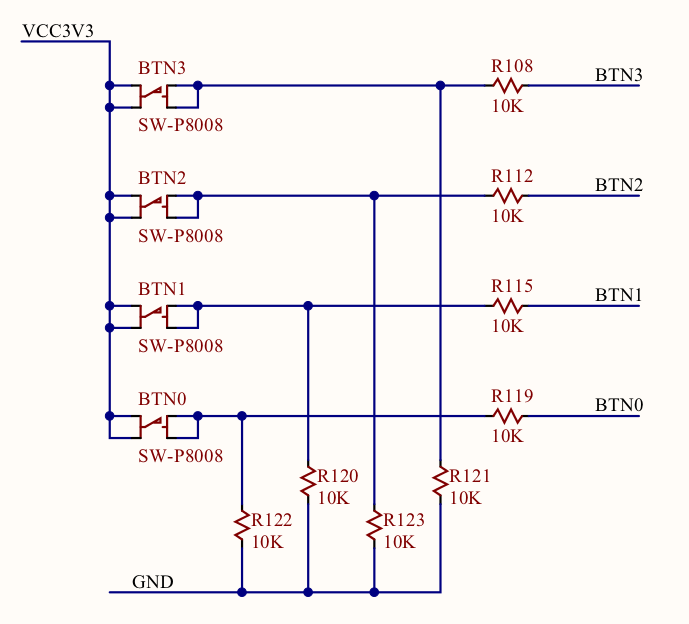
\includegraphics[width=0.5\textwidth]{btn1.png}
  \caption{Esquema provisto en el esquemático, 4 pulsadores.}
    \label{fig:btn}
\end{figure}

\begin{figure}[H]
  \centering
     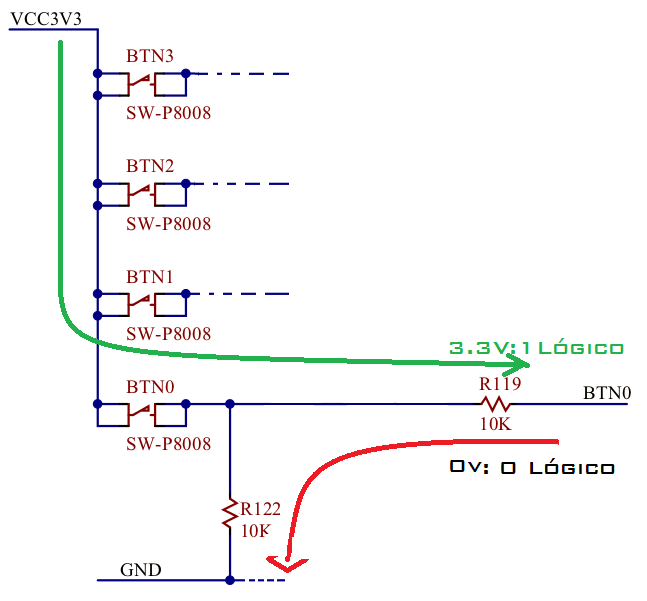
\includegraphics[width=0.6\textwidth]{btn2.png}
  \caption{Circulación de la corriente en el circuito, resistencia de 10k$\Omega$ protección contra cortocircuito}
      \label{fig:btn2}
\end{figure}
La figura \ref{fig:btn2} también muestra una configuración de un solo pulsador vemos la resistencia de pull down. Con colores hemos indicado el accionamiento del pulsador, tome como ejemplo \ref{fig:btn2}, el color rojo indica cuando el pulsador \textbf{BTN0} no ha sido presionado, esto indica que los pulsadores son de tipo \textbf{N.O} ó \textit{Normally Open in Low Mode} presentando un \textbf{0 lógico} a la salida, al presionar el pulsador, el contacto interno que este posee cierra el circuito conectándolo con la fuente de 3.3v como lo muestra el color verde de la figura \ref{fig:btn2}.
\subsection{Anti rebote por Software}
Resolver el problema de los rebotes de un pulsador puede ser una tarea fácil o compleja, la idea básica es \emph{muestrear} la señales de entrada de los pulsadores en un intervalo regular de tiempo para notar si hay cambios en la entrada, si no existieron cambios se debe mantener el estado actual del pulsador, si hay pulsos anormales debemos filtrar la señal. Después de realizar los cálculos correspondientes lo que decidimos implementar fue tomar un tiempo regular la señal producida por el pulsador para saber cuando la señal es verdadera, así que después de 5 millones de ciclos de reloj que corresponden aproximadamente a un tiempo de 110ms, si la señal se mantiene dejaremos pasar la señal del pulsador por la salida \emph{Q}, El modulo comentado se encuentra descrito en la seccion \ref{antirebote}

\begin{itemize}
	\item[Contador] Este contador  nos dirá cuanto tiempo ha pasado desde que la señal ha estado en alto, si la señal  ha estado en alto durante un tiempo definido por nosotros \textit{(50 mS)}, entonces es considerado como un pulso estable, y debería de setear la salida a 1. Esta aproximación es parecida vista en la implementación de \fnurl{DigiKey}{https://eewiki.net/pages/viewpage.action?pageId=4980758} pero más completa.
    \item[Registro 8bits] Esta aproximación es similar a la mencionada anteriormente, pero utiliza un registro de desplazamiento de 8bits en vez de un contador, lo que hace es ir desplazando los bits hasta alcanzar su valor máximo.
\end{itemize}

\subsubsection{Implementacion antirebote Vhdl} \label{antirebote}
\begin{listing}[H]
	\begin{minted}{vhdl}
library ieee;
use ieee.std_logic_1164.all;
use ieee.std_logic_unsigned.all;
entity counters_1 is
    port(CLK,btn_in: in std_logic;
         Q : out std_logic);
end counters_1;

--11100100111000011100000

architecture archi of counters_1 is
signal counter: std_logic_vector (23 downto 0) := (others => '0');

begin
    process (CLK, btn_in)
    begin
        if (CLK'event and CLK='1') then
				Q <= '0';
				IF counter > 0 and btn_in = '0' then
							counter <= counter + 1;
						end if;
		      IF (btn_in='1') THEN
					 IF (counter >= 5000000) THEN
						      Q <= '1';
								counter <= (others =>'0');
				    ELSE
					     counter <= counter + 1;
				    END IF;
				END IF;
			end if;
end process;
end archi;
\end{minted}
\caption{Implementacion Antirebote.}
\end{listing}
			
                


%Modulo Antirebote.
\clearpage
\newpage
\section{Modulo 2: Display de Siete Segmentos \label{sieteseg}}
\begin{figure}[H]
  \centering
     \includegraphics[scale=0.7]{mod7segmentos}
  \caption{Estructura del Modulo de 7 Segmentos.}
    \label{fig:catodo}
\end{figure}

Para desarrollar el modulo número dos del proyecto lo primero que realizamos es verificar en la hoja del fabricante las conexiones y el tipo de configuración utilizada en la placa de desarrollo \textbf{Nexys2}. Al revisar el Datasheet y manual encontramos que la placa contiene 4 displays de 7 segmentos y punto decimal(\textit{dp})  en la configuración de ánodo común lo cual implica que todos los ánodos de los leds que conforman el display este conectados a un punto en común como se aprecia en la figura \ref{fig:catodo} , para encender un solo led necesitaremos un valor lógico de \textbf{\textit{0}} para cerrar el circuito. 
\begin{figure}[H]
  \centering
     \includegraphics[scale=0.5]{img/catodo.png}
  \caption{Esquema Cátodo Común.}
    \label{fig:catodo}
\end{figure}
Revisando el esquemático de la tarjeta de desarrollo sabemos que la activación de los displays se da por la saturación del transistores pnp como se observa en la siguiente figura \ref{fig:esquema} :
\begin{figure}[H]
  \centering
     \includegraphics[scale=0.5]{img/configuracion.png}
  \caption{Esquema provisto en el esquemático, 4 pulsadores.}
    \label{fig:esquema}
\end{figure}
Los displays de 7 segmentos se encuentran en la configuración de ánodo común, un \textbf{0} se utiliza para encendido y un \textbf{1} para apagado (lógica negativa). Al representar los números usaremos una codificación de 4 bits que permiten los 10 dígitos (del \textit{0 al 9}),y así poder mostrar el dígito en un visualizador de siete segmentos siendo necesario decodificar el valor numérico según el patrón de LEDs indicado,  se tiene un carácter al cual se le asigna un valor numérico (codificación) para tratar con el digitalmente, posteriormente se transforma al patrón de LEDs correspondiente (de codificación) como se puede observar en el listing \ref{decodificador}. El número que se recibe en 4 bits codificado se decodifica a su valor correspondiente donde prenderemos o apagaremos los 8 leds del display.
\subsubsection{Implementacion Decodificador vhdl}
\begin{listing}[H]
	\begin{minted}{vhdl}
library IEEE;
use IEEE.STD_LOGIC_1164.ALL;
entity decoder_arch is
    Port ( numero : in  STD_LOGIC_VECTOR(3 downto 0);
           segment : out  STD_LOGIC_VECTOR(7 downto 0));
end decoder_arch;

architecture Behavioral of decoder_arch is

begin
	process(numero) begin
	case numero is
		when "0000" => segment <= "00000011"; --0
		when "0001" => segment <= "10011111"; --1
		when "0010" => segment <= "00100101"; --2
		when "0011" => segment <= "00001101"; --3
		when "0100" => segment <= "10011001"; --4
		when "0101" => segment <= "01001001"; --5
		when "0110" => segment <= "01000001"; --6
		when "0111" => segment <= "00011111"; --7
		when "1000" => segment <= "00000001"; --8
		when "1001" => segment <= "00001001"; --9
		when others => segment <= "11111111"; -- Nada
	end case;
end process;
end Behavioral;
\end{minted}
\caption{Decodificador de 4 bits.}
    \label{decodificador}
\end{listing}

\begin{table}[H]
\centering
\begin{tabular}{|c|c|}
\hline
\textbf{DECIMAL} & \textbf{BINARIO} \\ \hline
0                & 0001             \\ \hline
1                & 0001             \\ \hline
2                & 0010             \\ \hline
3                & 0011             \\ \hline
4                & 0100             \\ \hline
5                & 0101             \\ \hline
6                & 0110             \\ \hline
7                & 0111             \\ \hline
8                & 1000             \\ \hline
9                & 1001             \\ \hline
\end{tabular}
\caption{Valores Correspondientes de Binario a Bcd}
\label{binbcd}

\end{table}
Una vez hemos construido el modulo que se encarga de decodificar el valor  que queremos mostrar en los displays necesitamos saber como seleccionar el display adecuado; para esto utilizamos un multiplexor de 4 bits. un multiplexor o selector de datos es un circuito lógico que acepta varias entradas y solamente permite a una de ellas alcanzar la salida. La figura \ref{fig:mux} muestra el diagrama de un multiplexor, donde se observa que la salida Z puede tomar el valor de A o B, pero no de ambos a la vez, en base al valor del parámetro de selección $S0$. Nosotros hemos escrito el código que se encarga de recibir cual sera el modulo que seleccionemos \textit{(\textbf{selectorin})} una vez hecho esto lo que nosotros tenemos que hacer es habilitar con un 0 el display requerido y pasarle el valor decodificado El listing \ref{mux2}
\begin{figure}[H]
  \centering
     \includegraphics[scale=0.2]{img/MUX.png}
  \caption{Multiplexor 2 a 1.}
    \label{fig:mux}
\end{figure}

\subsubsection{Implementacion Multiplexor vhdl}
\begin{listing}[H]
	\begin{minted}{vhdl}
library IEEE;
use IEEE.STD_LOGIC_1164.ALL;

entity mux7s_arch is
    Port ( d0 : in  STD_LOGIC_VECTOR(3 downto 0);
           d1 : in  STD_LOGIC_VECTOR(3 downto 0);
           d2 : in  STD_LOGIC_VECTOR(3 downto 0);
           d3 : in  STD_LOGIC_VECTOR(3 downto 0);
           selectorin : in  STD_LOGIC_VECTOR(3 downto 0);
           numero : out  STD_LOGIC_VECTOR(3 downto 0));
end mux7s_arch;

architecture Behavioral of mux7s_arch is
begin
	process(selectorin,d0,d1,d2,d3) begin
		case selectorin is
			when "1110" =>
				numero<=d0;
			when "1101" =>
				numero<=d1;
			when "1011" =>
				numero<=d2;
			when "0111" =>
				numero<=d3;
			when others =>
				numero<=d0;
		end case;
	end process;

end Behavioral;

\end{minted}
\caption{Multiplexor usado en proyecto final.}
    \label{mux}
\end{listing}

Pero existe un problema y es que nosotros solo podremos visualizar un display a la vez, es decir tendremos que hacer un refresco por cada display de al menos \textbf{4ms} para engañar la retina del ojo humano utilizando la frecuencia correcta, se llega a la ilusión de que hay cuatro dígitos distintos y encendidos al mismo tiempo si son 4 displays en total sera \textbf{16ms}. Este efecto es similar al comentado por el profe Ramiro donde un vídeo esta compuesto de muchas imágenes sucesivas y a cierta frecuencia el ojo ve en movimiento. Una frecuencia de \textbf{250kHz} es más que suficiente para generar este efecto, por lo cual se utiliza el divisor creado en el modulo uno VHDL, que se presenta a continuación. 
\subsubsection{Implementacion de Modulo Selector Vhdl}
\begin{listing}[H]
	\begin{minted}{vhdl}
library IEEE;
use IEEE.STD_LOGIC_1164.ALL;
entity selector_arch is
    Port ( clk : in  STD_LOGIC;
           salida : out  STD_LOGIC_VECTOR(3 downto 0):="1110");
end selector_arch;
architecture Behavioral of selector_arch is

signal contador : integer range 0 to 200000 := 0;
signal ciclos : integer range 0 to 3 :=0;

begin
	process(clk) begin
		if rising_edge(clk) then
			if contador = 200000 then
				if ciclos = 0 then
					salida<="1101";
					ciclos<=ciclos+1;
					end if;
				if ciclos = 1 then
					salida<="1011";
					ciclos<=ciclos+1;
					end if;
				if ciclos = 2 then
					salida<="0111";
					ciclos<=ciclos+1;
					end if;
				if ciclos = 3 then
					salida<="1110";
					ciclos<=0;
					end if;
				contador<=0;
			else
				contador<= contador+1;
			end if;
		end if;
	end process;
end Behavioral;
\end{minted}
\caption{Modulo Selector,}
    \label{selector}
\end{listing}
\subsubsection{Integración Submodulos Siete Segmentos}
\begin{listing}[H]
	\begin{minted}{vhdl}
library IEEE;
use IEEE.STD_LOGIC_1164.ALL;

entity siete_segmentos is
    Port ( clk : in std_logic;
			  d0 : in  STD_LOGIC_VECTOR(3 DOWNTO 0);
           d1 : in  STD_LOGIC_VECTOR(3 DOWNTO 0);
           d2 : in  STD_LOGIC_VECTOR(3 DOWNTO 0);
           d3 : in  STD_LOGIC_VECTOR(3 DOWNTO 0);
			  salidacontrol : out std_logic_vector(3 downto 0);
			  salidanumero  : out std_logic_vector(7 downto 0));
end siete_segmentos;

architecture Behavioral of siete_segmentos is

component selector_arch is
    Port ( clk : in  STD_LOGIC;
           salida : out  STD_LOGIC_VECTOR(3 downto 0):="1110");
end component;

component mux7s_arch is
    Port ( d0 : in  STD_LOGIC_VECTOR(3 downto 0);
           d1 : in  STD_LOGIC_VECTOR(3 downto 0);
           d2 : in  STD_LOGIC_VECTOR(3 downto 0);
           d3 : in  STD_LOGIC_VECTOR(3 downto 0);
           selectorin : in  STD_LOGIC_VECTOR(3 downto 0);
           numero : out  STD_LOGIC_VECTOR(3 downto 0));
end component;

component decoder_arch is
    Port ( numero : in  STD_LOGIC_VECTOR(3 downto 0);
           segment : out  STD_LOGIC_VECTOR(7 downto 0));
end component;

signal salidaselector : std_logic_vector(3 downto 0);
signal salidamux : std_logic_vector(3 downto 0);
signal salidadecoder : std_logic_vector(7 downto 0);

begin
	modulo1: selector_arch port map(
				clk=>clk,
				salida=>salidaselector
				);
	modulo2: mux7s_arch port map(
				d0=>d0,
				d1=>d1,
				d2=>d2,
				d3=>d3,
				selectorin=>salidaselector,
				numero=>salidamux
				);
	modulo3: decoder_arch port map(
				numero=>salidamux,
				segment=>salidadecoder
				);
	salidacontrol<=salidaselector;
	salidanumero<=salidadecoder;

end Behavioral;


\end{minted}
\caption{x.}
    \label{mux2}
\end{listing}

Físicamente para realizar el impacto sobre la fpga debemos especificar cuales son las conexiones físicas en la fpga\footnote{Este fue uno de nuestros problemas al impactar pues al momento de mapear los pines reales olvidamos pinear nuestra señal de reloj.}, ademas también están especificadas en la tarjeta. véase figura \ref{Sw1} , figura \ref{Sw2}.
\begin{figure}[H]
  \centering
     \includegraphics[scale=0.4]{img/sws.png}
  \caption{Esquema provisto en el esquemático, 4 pulsadores.}
    \label{Sw1}
\end{figure}
\begin{figure}[H]
  \centering
     \includegraphics[scale=0.5]{img/sws.jpg}
  \caption{Esquema provisto en el esquemático, 4 pulsadores.}
    \label{Sw2}
\end{figure}

\subsection{Errores Comunes}
En este modulo tuvimos muchos problemas, apesar de ser sencillo en la fiscalización algunas veces siempre nos aparecía conexiones indefinidas y desconectadas. Toco realizar una revisión exaustiva de todo el código, para determinar por que no se conectaban.
Tiempo después al querer impactar en la fpga olvidamos pinear la señal mas importante de todas que es la que sincroniza todas las operaciones, hablamos de la señal del CLK. 

%Toolset.
\clearpage
\newpage
\section{Modulo 3: Protocolo RS232 \label{comunicacion}}

En la actualidad existen una gran cantidad de formas de comunicación que hacen que sea posible el intercambio de datos entre 2 o más dispositivos electrónicos, para que esto suceda los dispositivos deben elegir un protocolo el cual permiten establecer los parámetros de la misma. El protocolo \emph{Rs232} también conocido como EIA/TIA RS-232C designa una norma para el intercambio de datos binarios que se enviaran en forma serial, este tipo de comunicación en serie implica el envío de una serie de pulsos digitales de ida y vuelta entre dispositivos a una velocidad de transferencia mutuamente acordada.

Con el fin de hacer una comunicación serial, los dos dispositivos deben ponerse de acuerdo en los siguientes parámetros:
\begin{enumerate}
\item Velocidad a la que se envía, y leen los datos.
\item Los niveles de tensión que representan un 1 o un 0.
\item El significado de los niveles de tensión; Nivel de tensión alto es un \textbf{1} y un nivel de  tensión bajo representa un \textbf{0}, o lógica inversa.
\end{enumerate}

\begin{figure}[H]
  \centering
     \includegraphics[scale=0.7]{img/x.jpg}
  \caption{Interfaz Serial Usb-Db9.}
    \label{fig:rsserial}
\end{figure}

Para la comunicación entre ambos, ademas de los parámetros mencionados anteriormente es necesario usar una interfaz serial, en el mercado hay varias soluciones que se adaptan dependiendo el tipo de puerto y entrada por la cual enviaremos, como se muestra en la figura \ref{fig:rsserial}  la solución también se puede embeber en el mismo cable.

Una interfaz rs232 físicamente requiere :
\begin{itemize}
\item Una conexión a tierra común, ambos dispositivos tienen un punto de referencia.
\item Un cable para el remitente para enviar datos al receptor (línea de transmisión para el remitente conocido como \textbf{TX}).
\item Un cable para el remitente para recibir datos  (línea de recepción conocido como \textbf{RX}), véase la figura\ref{fig:hard}. \fnurl{SparkFun}{https://learn.sparkfun.com/tutorials/serial-communication}.
\end{itemize}
\begin{figure}[H]
  \centering
     \includegraphics[scale=0.6]{img/comunicacion.png}
  \caption{Hardware necesario para conexión asíncrona.}
    \label{fig:hard}
\end{figure}

Para realizar el envió de comunicación el protocolo rs232 sigue una maquina de estado que se resume en los siguientes pasos:
\begin{enumerate}
\item El transmisor envía un \textbf{"idle" (="1")}  cuando esta en reposo.
\item El transmisor enviara un bit de inicio \textbf{"start" (="0")} que indica el comienzo de la transmisión de datos.
\item Se envían los 8 bits de información
\item El transmisor envía un bit que indica la parada de cada byte.\textbf{"stop" (="1")} \footnote{Véase la figura \ref{fig:senal}}
\end{enumerate}

\begin{figure}[H]
  \centering
     \includegraphics[scale=0.6]{img/xx.png}
  \caption{Hardware necesario para conexion asincrona.}
    \label{fig:senal}
\end{figure}
Para desarrollar este modulo se crearon dos partes , la del receptor y el transmisor, cada uno se encarga de su tarea de enviar los datos serializado, recibirlos. 

El código implementado se presenta en las secciones de código \ref{rx}, \ref{tx}.

\subsubsection{Implementacion submodulo de transmisión Vhdl}
\begin{listing}[H]
	\begin{minted}{vhdl}
library IEEE;
use IEEE.STD_LOGIC_1164.ALL;
use IEEE.STD_LOGIC_ARITH.ALL;
use IEEE.STD_LOGIC_UNSIGNED.ALL;
entity tx_arch is
	Port (  clk : in  STD_LOGIC;
			  clk_enable: in STD_LOGIC;
           tx_start : in  STD_LOGIC:='0';
           tx_data : in  STD_LOGIC_VECTOR(7 downto 0);
			  tx : out  STD_LOGIC:='1');
end tx_arch;
architecture Behavioral of tx_arch is

type state is (idle,data,parity_state,stop1,stop2);
signal tx_state : state:=idle;
signal tx_data_temp    : std_logic_vector(7 downto 0);
signal tx_parity_bit   : std_logic;
signal tx_data_counter : integer range 0 to 7:=0;
constant uart_start  : std_logic :='0';
constant uart_idle   : std_logic :='1';

begin
	process(clk,clk_enable) begin
		if rising_edge(clk) then
			if clk_enable = '1' then
				case tx_state is
					when idle=>
						if tx_start = '1' then
							tx <= uart_start;
							tx_data_temp<=tx_data;
							tx_state <= data;
							tx_parity_bit <='0';
						else
							tx<=uart_idle;
						end if;
					when data=>
						tx <= tx_data_temp(tx_data_counter);
						tx_parity_bit <= tx_parity_bit xor tx_data_temp(tx_data_counter);
						if tx_data_counter = 7 then
								tx_state<=parity_state;
								tx_data_counter<=0;	
						else
							tx_data_counter<=tx_data_counter+1;
						end if;
					when parity_state=>
						tx <= tx_parity_bit;
						tx_state <=stop1;
					when stop1=>
						tx <=uart_idle;
						tx_state<=stop2;
					when stop2=>
						tx <=uart_idle;
						tx_state<=idle;
				end case;
			end if;
		end if;
	end process;

end Behavioral;
\end{minted}
\caption{Modulo de Transmision TX uart.}
    \label{tx}
\end{listing}

\newpage
\section{Modulo 4: Aplicacion de Escritorio \label{aplicacion}}


En este modulo desarrollamos el aplicativo utilizando como lenguaje de programación \emph{python} que posee soporte para el manejo de comunicaciones utilizando el protocolo rs232, la librería estándar se llama \textbf{\textit{pyserial}}, específicamente para nuestro desarrollado utilizamos la siguientes opciones:
\begin{enumerate}
\item 8 bits \textbf{serial.EIGHTBITS}
\item 2 bits de parada \textbf{serial.STOPBITS\_TWO}
\item paridad impar \textbf{serial.PARITY\_ODD}
\item velocidad de \textbf{9600} baudios.
\end{enumerate}

para nosotros simular el envió de comunicación serial lo realizamos en dos sistemas operativos para windows  utilizamos un emulador de puertos \emph{Virtual Serial Port en modo pair} que nos permite crear virtualmente puertos/dispositivo que utilizara el protocolo RS232. 
En Gnu-Linux utilizamos \textbf{socat}, un emulador multipropuesta que permite crear dispositivos de comunicaciones virtuales unidireccionales.
la forma de crear dos dispositivos en Linux es :
\begin{listing}[H]
	\begin{minted}{python}
socat -d -d  pty,raw,echo=0 pty,raw,echo=0
\end{minted}
\caption{Creacion de dos dispositivos ubicados en \textbf{/dev/pts/2, /dev/pts/3}.}
    \label{socats}
\end{listing}

En este sistema se debe agregar las siguientes librerías a pyserial para poder abrir y acceder al puerto serial : \textbf{rtscts=True,dsrdtr=True}

La idea principal de este modulo era simular como seria la integración entre el hardware y el aplicativo que se desarrollo, nosotros el aplicativo lo dividimos principalmente en 3 módulos, escritos en 3 scripts diferentes de python  que son : 
\begin{enumerate}
\item \textbf{Generador de Turnos}: Es un script en python que se encarga de generar los turnos solicitados por el usuario
\item \textbf{ModuloA,B}: Es es el aplicativo al que tienen acesso los asesores o mesas que resuelve el turno. 
\item \textbf{Visualizador de Turnos(\textit{Turnero})}: Es el que se encarga de mostrar el turno actual en pantalla para el publico.
\end{enumerate}
Para la interfaz gráfica se utilizo las librerías que dispone python como \textbf{pygame} el cual nos permite de una manera simple y rápida crear ventanas y entornos.
\begin{figure}[H]
  \centering
     \includegraphics[scale=0.38]{img/aplicativo.png}
  \caption{Esquema de Conexión Aplicación Web.}
    \label{fig:senal}
\end{figure}

\begin{listing}[H]
	\begin{minted}{python}
# -*- coding: utf-8 -*-			
import pygame		#Importar libreria necesaria
import serial
ANCHO=400			#Dimensiones de la ventana
ALTO=400	
BLANCO=(255,255,255)#constante de colores
ROJO=(255,0,0)
VERDE=(0,255,255)
AZUL=(0,0,255)
NEGRO=(0,0,0)

pygame.init()		#objeto que inicializa el entorno	
pantalla=pygame.display.set_mode([ANCHO,ALTO])#creamos ventana
pygame.display.set_caption("Generador De Turnos") 
\end{minted}
\caption{Creación  de ventanas en todos los scripts.}
    \label{window}
\end{listing}
Teniendo en cuenta esto para cada script lo que nosotros hemos realizado en nuestra aplicación simulada es que el usuario una vez presione la tecla \textbf{n}  utilizamos la opción de eventos que ofrece pygame y enviamos esto por serial a nuestro visualizador. 

\begin{listing}[H]
	\begin{minted}{python}
	for event in pygame.event.get():
			if event.type == pygame.QUIT:
				fin=True
			elif event.type ==	pygame.KEYUP:
				if event.key == pygame.K_n:
					if activado==0:
						#serial
						x=s.write(turn)
						print ("Envio : -- nuevo turno ")
						#pygame
						activado=1
						turnos+=1
						if turnos==100:
							turnos=1
\end{minted}
\caption{Gestión de eventos, presión de teclas .}
    \label{presion}
\end{listing}
Una vez se detecta el evento de la tecla enviamos esto el numero de turno generado. 

\begin{figure}[H]
  \centering
     \includegraphics[scale=0.5]{app}
  \caption{Turnero.}
    \label{fig:turnero}
\end{figure}

%Modulo Antirebote.
\clearpage
\newpage
\section{Anexos}
Los archivos adjuntos a este informe se encuentran en el repositorio del \fnurl{grupo.}{https://github.com/heticor915/DigitalElectronicsLab/tree/master/Reports/Final/Code} junto a su informe, su código se encuentra en este archivo en la sección de integración. 

Los archivos en  \LaTeX  correspondientes también se encuentran allí respecto a cada modulo desarrollado. La figura \ref{fig:treee} presenta la estructura que se encuentra en el repositorio.


\begin{figure}[H]
  \centering
     \includegraphics[scale=0.7]{tree}
  \caption{Arbol de Archivos Repositorio Github.}
   \label{fig:treee}   
\end{figure}

\clearpage
\newpage
\section{Agradecimientos}
Agradecimientos al profesor Ramiro por su paciencia, y sus sabias explicaciones a la hora de impactar la fpga, realizar los testbench, a los compañeros que nos apoyaron con sus ideas y aportes, a la universidad por permitirnos las instalaciones para realizar el desarrollo de este proyecto. 



\end{document}
